 \documentclass{article} %A4
\usepackage[a4paper,left=1.9cm, right=2.1cm,top = 1.2cm,bottom=2.3cm]{geometry}
\usepackage[utf8]{inputenc}%Umlaute
\usepackage[ngerman]{babel} %Texttrennung
\usepackage{graphicx}	%Grafiken
\usepackage{amssymb}
\usepackage{amsmath}
\usepackage{url}

\usepackage[labelformat=empty]{caption}
\title{Zusammenfassung - Web 2.0}
\author{
	Andreas Ruscheinski,
	Marc  Meier,
	Christian D.
}

\begin{document}
\maketitle
\tableofcontents
\section{Definitionsversuche}
	\subsection{Social Media, Enterprise 2.0, Web 2.0}
	\begin{itemize}
	\item\glqq Social Media bezeichnen digitale Medien und Technologien (vgl. Social Software), die es Nutzern ermöglichen, sich untereinander auszutauschen und mediale Inhalte einzeln oder in Gemeinschaft zu erstellen.\grqq (Wikipedia)\\
	\item\glqq Enterprise 2.0 bezeichnet im engeren Sinn den Einsatz von sozialer Software zur Projektkoordination, zum Wissensmanagement und zur Innen- und Außenkommunikation in Unternehmen\grqq (Wikipedia)\\
	\item\glqq Web 2.0 ist ein Schlagwort, das für eine Reihe interaktiver und kollaborativer Elemente des Internets, speziell des World Wide Webs, verwendet wird. Dabei konsumiert der Nutzer nicht nur den Inhalt, er stellt als Prosument selbst Inhalt zur Verfügung.\grqq (Wikipedia)
	\item Neue Technologien werden als Enabler gesehen d.h. Technologie ist Grundlange für die Unterstützung im Business Umfeld
	\item Verschiedene Modelle für die Beschreibung von Social Media, Enterprise 2.0, Web 2.0:
		\begin{itemize}
			\item Social Media Honeycomb
			\item SLATES
			\item FLATNESSES
		\end{itemize}
	\end{itemize}
	\subsubsection{Social Media HoneyComb}
	\begin{center}
	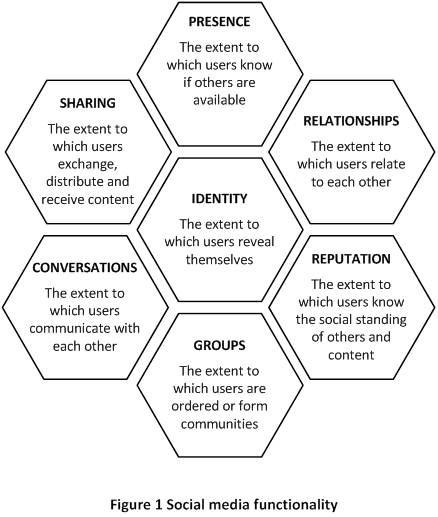
\includegraphics[scale=0.5]{img/SMHC_functionality.jpg}
	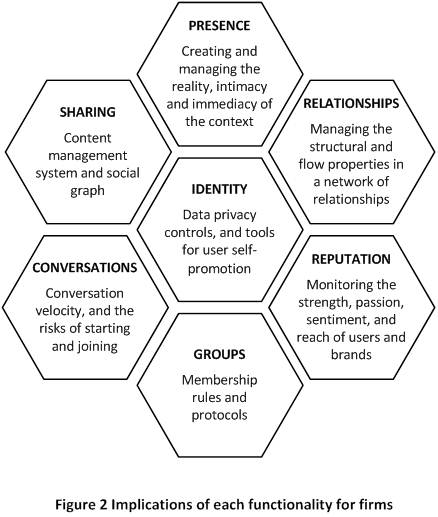
\includegraphics[scale=0.5]{img/SMHC_implications.jpg}
	\end{center}
	\begin{itemize}
		\item Charackterisierung möglich durch aus Wahl verschiedener Waaben als Baublöcke
		\item Hauptwaabe = Hauptaufgabe, Nebenwaaben = Zusätzliche Möglichkeiten
	\end{itemize}
	\subsubsection{SLATES}
	\glqq SLATES is an initialism that describes the business impacting capabilities, derived from the effective use of Web 2.0 technologies in and across enterprises.\grqq (Wikipedia), Jedes Element beschreibt eine zentrale Komponente von Enterprise 2.0
	\begin{description}
		\item[SEARCH] Unterstütze die unternehmensweite Suche nach Inhalten;
		Finden, was das Unternehmen weiß und in welchen Köpfen
		\item[LINKS] Ähnliches verbinden nach Assoziationen und Gemeinsamkeiten;
		Abkehr vom  "Teile und herrsche"
		\item[AUTHORSHIP] Niedere Barrieren für Authorship;
		Jeder kann und soll sich als Autor kreativ einbringen
		\item[TAGS] Jeder kann dem Wissen seine Strukturen überstülpen;
		Emergente Strukturen lösen starren Hierarchien und Schemata ab
		\item[EXTENSIONS] Erweiterung der eigenen Sicht und Bewertung;
		Empfehlungssysteme, Bewertungsportale
		\item[SIGNALS] Push und Pull durch Signal-basierte Kanäle ersetzen
	\end{description}
	\subsubsection{FLATNESSES}
	FLATNESS ist eine Erweiterung für SLATES basieren auf der Beobachtung von Enterprise 2.0 in Action. Einige Beobachtungen:
	\begin{itemize}
		\item Enterprise 2.0 is going to happen in your organization whether you
		like it or not
		\item Enterprise 2.0 doesn’t seem to put older IT systems out of business
		\item the benefits of Enterprise 2.0 can be dramatic, but only build steadily
		over time
	\end{itemize}
	\begin{center}
		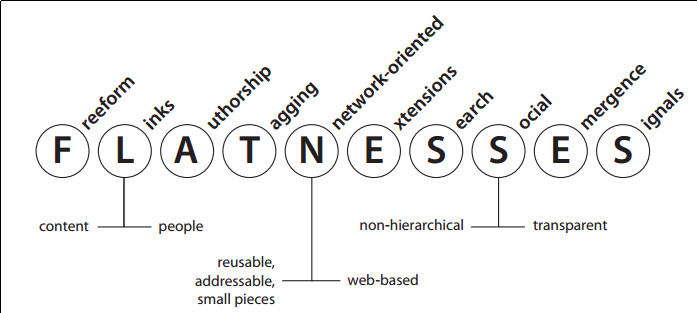
\includegraphics[scale=0.5]{img/FLATNESS.jpg}
	\end{center}
	\subsection{Vergleich Enterprise 1.0 und Enterprise 2.0}
	\begin{center}
		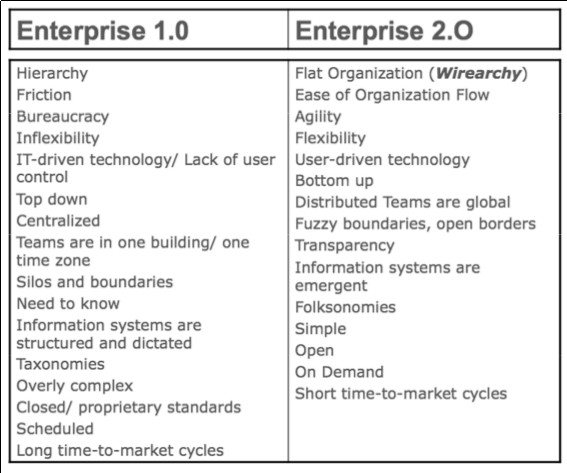
\includegraphics[scale=0.8]{img/CompareW1W2.jpg}
	\end{center}
	\subsection{Konzepte}
	\begin{itemize}
		\item Entwicklung des Web 2.0 führte zu einer Reihe neuer Ansätze
		\begin{description}
			\item[User Interface:] Lightweight Rich Client, Ajax, Desktop Feel
			\item[Content:] User Generated Content, Prosumer
			\item[Cooperation:] Wisdom of Crowd, Crowd Sourcing
			\item[Economy:] Attention, Intention, Network Economy
			\item[Life Cycle:] Perpetual Beta, Consumer designed product
			\item[Social Media:] facebook usw...
		\end{description}
		\item zentrale Merkmale: Interaktion, Kollaboarion, Sharing, User Generated Content
	\end{itemize}
	\subsubsection{Anwendungen - User Generated Content}
	Der Inhalt wird durch den User erstellt. Mögliche Kategorisierung von Web 2.0 Anwendungen:
		\begin{description}
			\item [Upload Content:] Der Benutzer lädt den Inhalt einer Webseite hoch, Bsp: Youtube, Flickr
			\item [Complete User Dominance:] Der Benutzer ist zentrales Element der Webseite, Bsp: Foren, Blogs, Wikis, Twitter
			\item [Trust Themen:] ???
			\item [Kollaboration:] Die Benutzer arbeiten Zusammen, Bsp: Google Docs, Etherpad $\rightarrow$ Prosumers
		\end{description}
	\subsubsection{Anwendungen - Cooperation Portals}
	Ein Unternehmen stellt ein ????. Mögliche Kategorisierung von Coopartion Portale:
		\begin{description}
			\item[Business Networks:] Plattform für den Austausch von unternehmesrelevanten Informationen, Bsp: XING; LinkedIn
			\item[Interest Networks:] Plattform für den Austausch von Interessen der Benutzer, Bsp: Facebook, MySpace
			\item[Synchronization:] Plattform für die Synchronization von Benutzerinformationen über verschiedene Endgeräte, Bsp: Foxmarks(Lesezeichen), Plaxo(Kontaktdaten)
		\end{description}
	\subsubsection{Technologien - Konzepte}
	\begin{description}
		\item[Advanced Javascript:] Einsatz von komlexen Javascript Programmen für die Realisierung der Webseite
		\item[AJAX,XHR,HTML5:]  Realisierung einer dynamischen Webseite durch asynchrone Kommunikation
		\item[Folkonomies und Tags:] Webseite stellt eine Benutzer definierte Möglichkeit für die Organisation der Daten, Bsp: Hashtag, Subreddit
		\item[Browser Extensions und Plugins:] Erweiterung der Browser durch den Anwendungsentwickler, dadurch Desktop Look-and-Feel
		\item[Probabilistische Algortihmen (Bitcoin):] Einsatz von Probablistischen Algorithmen auf verteilter Basis für die Erbrining einer Leistung, Bsp: Bitcoin(Online Wallet)
	\end{description}	
	\subsubsection{Technologien - Werkzeuge}
	\begin{description}
		\item[JS Libraries:] jQuery, extJS, Angular
		\item[Embedded JS:] Einsatz von Javascript auf Server/Desktop Ebene, Bsp: V8, node.js
		\item[Ajax KITS:] Implementierung für die asynchrone Kommunikation, Bsp: Rico, Dojo, GWT
	\end{description}
	\subsection{Notizen}
		\begin{itemize}
			\item Silos and Boundaries
				\begin{itemize}
					\item Problem bei nicht-Silos: Snowden $\rightarrow$ Daten werden selbstständig
					\item Silos sind alles an Daten, die in einem Umfeld formatiert sind, die man aber irgendwann nicht mehr interpretieren kann $\rightarrow$ sie werden inkompatibel
					\item Wünschenswert: Migration von bspw. Facebook zu MySpace
				\end{itemize}
				\item Prosumers: Nutzer in der Doppelrolle \glqq Inhalt von allen für alle\grqq
				\item Die Daten-Sammel-Phase ist zuende $\rightarrow$ wie sollen sie verarbeitet werden? $\rightarrow$ Google weiß bspw. schon vorher ob eine Grippewelle eintritt
		\end{itemize}
	\section{AJAX und Web 2.0}
	\subsection{Allgemein}
	\begin{itemize}
		\item AJAX ist KEINE neue Technologie sondern Design Pattern
		\item Problem: Verhalten des Benutzers anders als bei Desktop Anwendungen
		\begin{itemize}
			\item Blättern durch einzelne Seiten
			\item Wenig Interaktivität 
			\item Kein undo/redo
			\item Viele Unklarheiten - Reload, Bookmarks und zurück
		\end{itemize}
	\end{itemize}
	\subsection{Vergleich der Reload Cycles}
	\begin{center}
		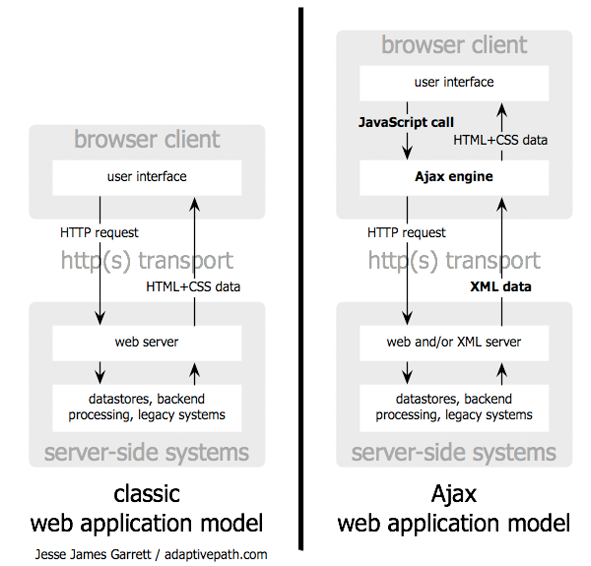
\includegraphics[scale=0.5]{img/HTTP_Ajax.png}
	\end{center}
	\subsection{AjaX}
	\begin{itemize}
		\item AjaX = Asynchronous Javascript XMLHTTPRequest
		\item Asynchron = GUI nicht blockiert während Übertragung
		\item kein neuer Seitenaufbau sondern dynamische Erweiterung mittels Javascript
	\end{itemize}
	\subsection{Konzepte und Technologien}
	\begin{itemize}
		\item Schwächer gekoppelte Kommunikation
		\begin{itemize}
			\item Asynchrone Kommunikation: XMLHttpRequest, Sockets
			\item Varianten der synchrone Kommunikation: Multipart MIME, Server Sockets
		\end{itemize}
		\item Leichtgewichtiges Processing in n-tier Denkweise
		\begin{itemize}
			\item Client-Side Scripting: Javascript
			\item Server-Side Code Generation: PHP, Java – basierte Ajax Kits
		\end{itemize}
		\item OO Dokumentenmodell mit Repräsentationsabtrennung
		\begin{itemize}
			\item Markup: HTML, XML, XHTML
			\item Repräsentations Transformation: CSS, XSLT
			\item DOM – Manipulation: innerHTML, JS DOM
		\end{itemize}
	\end{itemize}
	\section{Wirtschaftliche Aspekte}
	Einfach mal in den Folien lesen \glqq02-netzwerk-effekte-2015-bw.pdf\grqq
	\section{XMLHttpRequest}
	\subsection{Allgemein}
	\begin{itemize}
		\item XMLHttpRequest ist ein JS Objekt, REQUEST öffnet HTTP Verbindung, RESPONSE verwaltet die Antwort
		\item Allgemeines Vorgehen:
		\begin{enumerate}
			\item Neues XMLHttpRequest-Objekt erstellen
			\item Request spezifizieren: TYP(GET,POST,PUT,DELETE,\dots),URL (ggf. mit Query Encoding), Boolean Asyc (True für Asynchrone Kommunikation, False für Synchrone Kommunikation)
			\item Setzen des Event Handlers (eine Funktion), welche Ausgeführt wird wenn Antwort vom Server kommt
			\item Senden des Request ggf. mit Body (bei POST leer)
		\end{enumerate}
		\item GET ist relativ unsicher(leicht einsehbar, gilt nicht bei XHR), ggf. Problem mit Firewalls (Empfohlen wenn wenig Daten im Query)
		\item POSTS werden nicht gecached und nervige Browsermeldung(nicht bei XHR) (Empfohlen bei vielen Daten im Query)
		\item Synchron (nicht Ajax): sinnvoll wenn die Interaktion des Users zu verhinden (Bsp.: online Banking)
		\item Asynchron: Programieraufwand (Timeout, Fehlerfall, Mehrfach-Requests, Anzeige an die User über laufenden Ladevorgang)
	\end{itemize}
	\section{Bitcoin}
	\subsection{Allgemein}
	\begin{itemize}
		\item \glqq Geld ist ein \textbf{Recht} zur Ausführung einer bestimmten Transaktion das von seinem \textbf{Träger} \textbf{genau einmal ausgeübt} werden kann und \textbf{nur durch} die Ausübung auf \textbf{andere übergeht}.\grqq
		\item \glqq Träger:\grqq
		\begin{itemize}
			\item an Name gebunden
			\item an Kenntnis gebunden
			\item an Pseudonym gebunden
			\item an den Besitz eines Objekts gebunden
			\item an Körper gebunden
		\end{itemize}
		\item \glqq Genau einmal ... von seinem Träger \grqq
		\begin{itemize}
			\item Geld kann nicht mehrfach Ausgegeben
			\item Weitergabe möglich
			\item Backup möglich
		\end{itemize}
		\item \glqq Nur durch\grqq
		\begin{itemize}
			\item Kein Erzeugung des Geldes ohne Deckung
			\item Gegenleistung in Zeit, Energie, Gold (Wert-Deckung)
			\item Gesellschaftlich Befugnis (Regelungs-Deckung)
			\item Gesellschaftliche Akzeptanz (De Facto Deckung)
		\end{itemize}
		\item \glqq auf andere übergeht\grqq
		\begin{itemize}
			\item einer verliert,einer bekommt das recht
		\end{itemize}
	\end{itemize}
	\subsection{Was ist Bitcoin?}
	\begin{itemize}
		\item Träger des Geldes
		\begin{itemize}
			\item Bindung an Pseudonym (Bitcoin Adresse)
			\item Nachweis der Befugnis durch Key Paar
			\item Bitcoin Adresse ist hash des public key
			\item Private Key verlieren ist Geld verlieren
		\end{itemize}
		\item Übertragung
		\begin{itemize}
			\item Peer-to-Peer
			\item jeder Teilnehmer betreibt Bitcoin Knoten
			\item jeder Knoten speichert Konto-Stände aller Adressen
			\item Transaktion an alle Knoten gesandt
			\item Berechtigugn wird durch Signatur überprüft
			\item neue Konto-Stände werden an alle Knoten gesandt
			\item Problem: Inkonsistente Konto-Stände (einige Knoten sind noch nicht über neue Kontostände informiert)
			\item Lösung: Bitcoin Blockketten-Algorithmus
		\end{itemize}
	\end{itemize}
	\subsection{Zusammenfassung nach Khan Academy}
	Dieser Abschnitt stammt von Marc.
	Die Infos wurden den Lehrvideos der Kahn Academy \url{https://www.khanacademy.org/economics-finance-domain/core-finance/money-and-banking/bitcoin} entnommen.
	Alle Unterabschnitte entsprechen im wesentlichen Zusammenfassungen der Videos
	\subsubsection{What is it \& Overview}
	Diese Videos bieten eine Einführung zu Bitcoin.
	Es werden ein paar Grundlagen und Vorteile genannt, diese folgen hier eventuell später.
	\subsubsection{Cryptografic hash functions \& Digital signatures}
	Die Inhalte dieser Videos sollten Grundlagen für Informatiker darstellen.
	Auf das Wichtigste heruntergebrochen sind diese:
	\begin{itemize}
		\item Kryptografische Hash-Funktionen sind mathematische Funktionen, die einen Wert (Message;variable Länge) auf einen anderen Wert (Hash, Digest, Tag;feste Länge) abbilden.
		\item Die wichtigsten Eigenschaften sind effiziente Berechenbarkeit, Kollisionsresistenz, Rückschluss auf Eingabe nicht möglich und Streuung der Werte (1 Bit in Eingabe geändert heißt nicht, dass die Ausgaben ähnlich sind)
		\item Bekannte Vertreter sind MD5 und SHA-256
		\item Zum Digitalen Signieren hat ein Teilnehmer ein public-private-Schlüssel-Paar
		\item Eine zu signierende Nachricht wird gehashed und mit dem privaten Schlüssel verschlüsselt, heraus kommt die digitale Signatur, welche Autor und Nachricht bestätigt.
		\item Zum Überprüfen wird die Signatur mit dem öffentlichen Schlüssel entschlüsselt, der entstehende Wert kann mit dem Hash der empfangenen Nachricht verglichen werden.
		\item (Kleines, da schwieriges/unwahrscheinliches) Problem: Aufgrund von Kollisionen (mehrere Nachrichten können selben Hashwert haben) keine 100-prozentige Sicherheit!
	\end{itemize}
	\subsubsection{Transaction records}
	In diesem Video habe ich noch einige Verständnisprobleme, daher wäre eine Sichtung nochmal gut.
	Insbesondere die Unterscheidung Teilnehmer und Transaktion ist mir irgendwie noch nicht zu 100 Prozent klar.
	\begin{itemize}
		\item Bitcoin-Datenbank speichert nicht die Werte einzelner Konten, sondern viel eher die Transaktionen der Bitcoins
		\item Teilnehmer durch Bitcoin-Adresse oder Pseudonym repräsentiert. 
		Diese(s) entspricht einem öffentlichen Schlüssel (eines privat-public-Key-Paares).
		Das bedeutet, dass so eine Adresse ohne zentrale Instanz selbst generiert werden kann, jedoch auch, dass eine (unwahrscheinliche, da $2^256$ Adressen) Kollisionsmöglichkeit besteht.
		Achtung: Im Skript handelt es sich bei der Bitcoin Adresse um den Hash des Schlüssels!
		\item Das Guthaben eines Teilnehmers setzt sich zusammen aus den vergangenen, noch nicht als ungültig (besseres Wort?) erklärten Transaktionen, für die der Teilnehmer eine Berechtigung (in Form eines private Key) hat.
		Beispiel: Alice hat Bob 10 BTC überwiesen, Carol hat Bob 15 BTC überwiesen.
		Beide Überweisungen sind irgendwo in der Historie zu finden.
		Bob hat 25 BTC.
		\item Bei einer Überweisung von 5 BTC von Bob an Dora schreibt Bob eine Transaktion.
		Diese enthält die Quellen, also beispielsweise die Transaktion von Alice an Bob (die besagt, dass Bob 10 BTC) besitzt; den Empfänger Dora (bzw deren public Key/Bitcoin-Adresse) und den Wert in Höhe von 5 BTC, sowie das Rückgeld an Bob (weil wir von einer 10 BTC Transaktion ausgehen, will Bob noch etwas wiederhaben).
		Die Transaktion wird von Bob signiert und an die Knoten weitergegeben, welche diese bestätigen sollen.
	\end{itemize}
	\subsubsection{Proof-of-work}
	Proof-of-work ist ein Verfahren, welches genutzt wird, um die Blockchain aufzubauen.
	Diese erklärung ist erstmal unabhängig von Bitcoin
	\begin{itemize}
		\item Zweck von Proof-of-work: Um einen Dienst zu nutzen (z.B. einen Block in die Blockchain zu hängen) muss zuerst großer rechnerischer Aufwand betrieben werden.
		Die Überprüfung muss sehr einfach funktionieren.
		\item Idee: Zu einer Challenge c soll ein Proof p gesucht werden, sodass der Hash h(c,p) mit mindestens einer bestimmten Anzahl von 0 beginnt.
		Das ist im Wesentlichen ein Brute-Force-Prozess
		\item Zum Überprüfen, ob p ein Proof zu c ist, muss lediglich h(c,p) ausgerechnet werden.
	\end{itemize}
	\subsubsection{Transaction block chains}
	\begin{itemize}
		\item Im vorletzten Abschnitt wurde eine Transaktion an die Knoten weitergegeben
		\item Die Knoten sammeln unabhängig voneinander Transaktionen und fassen diese zu Blöcken zusammen; das heißt die Transaktionen werden immer paarweise gehashed, bis lediglich ein einzelner Hash für den gesamten Block übrig ist.
		\item Ziel ist es, diesen Block an die Blockchain anzuhängen, also mit dem letzten aktuellen Block zu verknüpfen, welcher wiederum mit seinem Vorgänger verknüpft ist (bis zu einem ursprünglichen Genesis-Block)
		\item Die Verknüpfung von jetzigem Block mit dem aktuellsten Block in der Blockchain ist die Challenge. 
		Zu dieser soll ein Proof (letzter Abschnitt) werden.
		Wie viele Nullen dieser mindestens haben soll, wird vom Netzwerk festgelegt (nächster Abschnitt).
		\item Im Schnitt wird alle 10 Minuten ein solcher proof gefunden.
		Alle Knoten arbeiten an eigenen, unterschiedlichen Blöcken (da diese verschiedene Transaktionen enthalten können).
		\item Finden zwei Knoten (in etwa) gleichzeitig einen Proof zu ihrem Block, werden beide Blöcke an die Blockchain angehängt, es entsteht eine Verzweigung.
		Nachfolgende Blöcke sollen immer an die längste Kette angehängt werden.
		Achtung: Gemeint ist nicht die Anzahl der Blöcke, sondern die schwierigste Kette, also jene, welche die meisten "Anfangsnullen" enthält.
	\end{itemize}
	\subsubsection{The money supply}
	\subsubsection{The security of transaction block chains}
	\section{Ajax und Web 2.0 Sicherheit}
	\subsection{Allgemein}
	\begin{itemize}
		\item Motive der Angreifer
		\begin{itemize}
			\item Ausspähen von Daten
			\item Modifikation von Transaktionsdaten
			\item Installation von Mal- und Spyware
			\item Aktivieren von Bot-Netzen
			\item Schädigung von Personen bzw. Firmen
			\item Erzielen von Netzerk-Effekten
		\end{itemize}
		\item Was kann der Angreifer?
		\begin{itemize}
			\item Surfer eine Webseite des Angreifers laden
			\begin{enumerate}
				\item Javascript des Angreifers kommt zur Ausführung $\rightarrow$ Zugriff auf Client Ressourcen (Cookies, Formulardaten)
				\item Surfer glaubt sich auf einer anderen Seite $\rightarrow$ PIN angegeben, da ja auf Bankseite bin
				\item Cross Site Request auf eingebettete Objekte kommt zur Ausführung $\rightarrow$ Autorisierungs-Cookie wird an nicht-intendierten Link gesendet
				\item Lancieren gezielter Angriffe $\rightarrow$ Image / Video / PDF, das einen Zero Day im PlugIn / Player ausnutzt
			\end{enumerate}
			\item Den Content Provider zu einem Einbinden eigener Scripte verleiten (Problem: Scripte haben maximale Rechte auf der Seite)
			\item Den Content Provider zu einem Setzen von Links verleiten 
			\item Eingabe spezielle formatierten Inputs 
		\end{itemize}
		\item Konzentation auf Cross Site Angriffe
		\item Weitere Probleme: Soziale Probleme des Mitmach Models (Multible Identitäten)
	\end{itemize}
	\subsection{Sicherheitsmodelle für mobilen Code}
	\begin{itemize}
		\item Problem: Mobiler Code = Ausführebare Datei, die vom Server geladen wird
		\item Lösungen: Sandbox, Signierter Code, Policy Files
	\end{itemize}
	\subsubsection{Sandbox}
	\begin{itemize}
		\item Mobiler Code läuft in Sandbox und verhindert dadurch Zugriff auf lokale Ressourcen 
		\item Problem: ggf. zu weite Eingrenzung der Rechte (keine clientseitige Persistenz), kein kontrolliertes Durchbrechnen möglich
	\end{itemize}
	\subsubsection{Signierter Code}
	\begin{itemize}
		\item Code wird durch Instanz signierte, Signierter Code erhält weitergehende Rechte
		\item Problem: Vertrauen an Drittinstitutionen, Unklar was weitergehende Rechte bedeuten, Nicht sinnvoll praktikabel (hoher Aufwand)
	\end{itemize}
	\subsubsection{Policy Files}
	\begin{itemize}
		\item User kann steuern, welche Rechte an das Script freigegeben werden (sehr Flexibel)
		\item Problem: ggf. zu kompliziert für User, nicht zero install
	\end{itemize}
	\subsection{Sicherheit von Javascript - Same Origin Sandbox}
	\subsubsection{Allgemein}
	\begin{itemize}
		\item Eingebundenes Javascript auf einer Seite von Seite X hat Lese/Schreib-Rechte auf den Dokumenten welche die selbe Herkunft (Seite X) haben
		\item selbe Herkunft ist verletzt gdw:
		\begin{itemize}
			\item Verschiedene Domäne in der URL
			\item Protokoll verschieden
			\item Port verschieden
			\item Ein Script von Rechnername, ein anderes von IP Adresse geladen
			\item Unterschiedliche Subdomänen
			\item Redirections
		\end{itemize}
		\item Durchbrechen der Sandbox Benutzerkontrolliert oder Systematisch nach definierten Standard(HTML5 File Reader/Writer)
		\item Schutzziele:
		\begin{itemize}
			\item Lokale Ressourcen: kein Zugriff auf Festplatte, Devices, Sensoren, Durchbruch nur systematisch
			\item Fremde Ressourcen: kein Zugriff auf den DOM/Formulardaten anderer Dokumente
			\item Remote Ressourcen: kein Zugriff fremde Domänen
		\end{itemize}
		\item Problem: ISP-Anomalität (www.myisp.com/dave/script1.js und www.myisp.com/john/script1.js können aufeinander zugreifen), document.domain Property (www.bsp.com und wiki.bsp.com können nicht interagieren $\rightarrow$ document.domain = \glqq bsp.com\grqq)
		\item XHR, localStorage und Web Messaging unter liegen Same Origin Restriktion
		\item Bilder, CSS und Skripte unterliegen \textbf{nicht} Same Origin Restriktion $righarrow$ dadurch Attacken möglich: Web Spoofing, GUI Redressing, Seiteübernehmen
		\item Websockets haben eigene Sicherheitsschicht
		\item Cooklies unterliegen browserseitigen Einstellungen
		\item Flash Cookies unterliegen browser- und Flash-Einstellungen
	\end{itemize}
	\subsubsection{Durchbrechen der Same Origin Sandbox}
	\begin{itemize}
		\item Durchbrechen durch Cross Site Zugriffe (???)
		\begin{itemize} 
			\item Möglich durch: Javascript, CSS, Requests
			\item Wenig Problem da Vermeidung durch geeigneten Webseiten Entwurf
		\end{itemize}
		\item Durchbrechen durch Entscheid des Browser-Herstellers
		\begin{itemize}
			\item Explorer: Durch OS Einstellungen, ActiveX/Flash Komponenten
			\item Firefox: Durch signed code, Plugins, Flash Komponenten
			\item Sollte man nicht nutzen, da plattformabhängig, öfters unsicher implementiert und
			oft geändert, unterschiedliche Mitwirkung des end-users erforderlich
		\end{itemize}
		\item Durchbrechen durch Protokoll-Erweiterung
		\begin{itemize}
			\item CORS = Cross Origin resource Sharing (W3C Standard)
			\item Web Messaging(HTML5)
			\item JsonRequest (???)
			\item JSONP (????)
		\end{itemize}
	\end{itemize}
	\subsubsection{CORS - Cross Origin Resource Sharing}
	\begin{itemize}
		\item ermöglich kontrolliertes Durchbrechen der Same Origin Sandbox durch Beteiligung des Servers
		\item erlaubt XHR auf andere Domäne 
		\item Nutzt ggf. Preflighting (HTTP OPTIONS Request) d.h. holt sicher Erlaubnis des Servers zur Abweichung vom üblichen Verhalten
		\item Preflighting wenn Methode nicht GET oder POST, Request body hat MIME Type != text/plain oder spezielle Header hinzugefügt
		\item Ablauf:
		\begin{enumerate}
			\item Server alice.com hat Daten
			\item Server bob.com will Daten von alice.com einbinden
			\item alice.com versieht Daten mit zusätzlichen Header
			\item Browser gestattet der Seite von bob.com ein XHR auf alice.com
		\end{enumerate}
		\item Alternative: Trust, bob vertraut alice, alice erlaubt bob die Nutzung (Headererweiterung)
		\item Client: alles wie immer :D
		\item Server: diverse neue Header, welche verarbeitet werden müssen
	\end{itemize}
	\begin{center}
		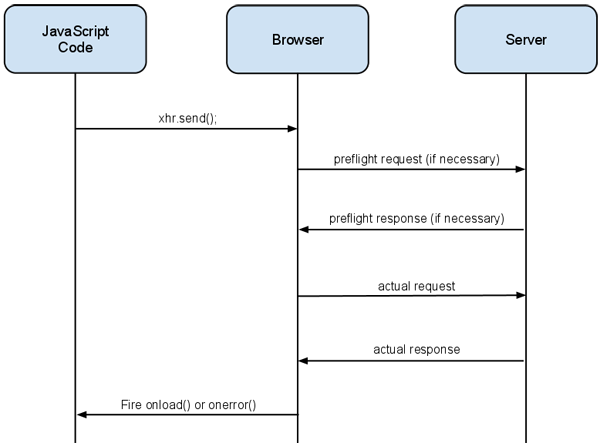
\includegraphics[scale=0.3]{img/CORS_FLOW.png}
	\end{center}
	\subsubsection{Web Messaging}
	\begin{itemize}
		\item Ermöglicht den Datenaustausch zwischen Dokumenten in anderen Tabs/Fenstern
		\item Senden: targetWindow.postMessage(message,targetURL)
		\item targetWindow = Referenz auf Zielfenster (Erhalt durch Öffnen des Fenster $\rightarrow$ return-Wert von window.open(); enthalten als contentWindow Property eines iframes)
		\item message = String oder Object das gesendet wird
		\item targetUrl = URL des Zielfensters
		\item Empfänger implementiert onmessage-Handler $\rightarrow$ erhält ein Event mit den Attributen data (Inhalt der Nachricht), origin (URL des Senders), source (Referenz auf das Sender-Fenster)
		\item Sicherheit
		\begin{itemize}
			\item Sender: Kann vertrauliche Daten an böses Ziel senden 
			\item Empfänger: Erhalte nicht vertrauenswürdige Daten aus böser Quelle
		\end{itemize}
	\end{itemize}
	\subsubsection{iframe Security}
	\begin{itemize}
		\item Inhalte können von Cross-Site über iframes eingebunden werden
		\item Problem: Fremde Site verändert eigene Site, Nutzer sieht nicht wer für den Inhalt verantwortlich, Site macht sich fremde Inhalte zu Nutze
		\item Lösung: sichtbar einbetten, iframe busting (Javascript der eingebetten Seite greift auf parent zu und schreibt sich auf höchster Ebene), Server setzt X-Frame-Options Header auf Deny (komplettes Verbot), Allow-From url (Einbinden wenn Basisseite bestimmte URL ist) oder Sameorigin (Einbinden nur wenn Basisseite same origin ist)
	\end{itemize}
	\subsubsection{Cross Site CSS}
	\begin{itemize}
		\item Einbinden von CSS von andere Seite
		\item Problem: Verdecken von Elementen, Unsichtbarkeit von Elementen, GUI redressing Attacken
	\end{itemize}
	\subsubsection{Cross Site Scripting}
	\begin{itemize}
		\item Definition: Webseite stammt aus einer Domain und lädt Skripte von einer anderen Domain
		\item WICHTIG: Cross Domain XHR verhindert durch Sandbox, Cross Domain Scripting wird nicht verhindert durch Sandbox
		\item Warum? Eigentlich wenig Sinn ausser bei Zugriff auf Mashup (Google Maps, Flickr Gallerie)
		\item Probleme: Fremdes Script zerstört Aussehen meiner Web Site völlig, Fremdes Script liest Werte aus Formularen aus

		\item Bookmarklet = ist ein kleines in JavaScript geschriebenes Makro, das als Bookmark abgespeichert wird und dadurch die Funktionen eines Webbrowsers erweitert; Problem: laufen mit den Rechten der aktuell angezeigten Seite und können so Cookies-Stehlen und remote-Code hinzufügen
	\end{itemize}
	\subsubsection{Cross Site Request Forgery}
	\begin{itemize}
		\item Angreifer plaziert IMG-Link auf einer Seite mit Link welcher aufgerufen wird wenn Seite geladen wird
		\item Bsp: $\le$img src=\glqq http://bank.example/withdraw?account=bob\&amount=1000000\&for=mallory\grqq$\ge$
		\item Verteidigung: 
		\begin{itemize}
			\item nutzen von Logoff (Anfragen werden verworfen da Benutzer nicht angemeldet)
			\item Service nur als POST anbieten
			\item Zur Autorisierung auch ein Hidden Field nutzen
			\item Cookie double submission: Cookie und dazupassenden Teil in einem hidden field erwarten
		\end{itemize}
		\item Probleme:
		\begin{itemize}
			\item Cookies zur Vermittelung von Rechten (bei Aufruf wird Cookie verstandt); Erwünscht: Cross Domain User Tracking (Marketing), Unerwünscht: weil Cookies auch zum Speichern von User Credentials benutzt werden
			\item 2 implizite Annahmen im Link-Konzept: User sieht den Link, auf den er klickt aber er sieht nur Inhalt des Link-Tags nicht die URL $\rightarrow$ Betrug durch falsche GUI Konstruktion; User kennt den Effekt des Links, auf den er klickt aber URL namens abbuchen.php muss nicht abbuchen $\rightarrow$ Betrug durch vorgespiegelte URL Semantik
		\end{itemize}
	\end{itemize}
	\subsection{Konzeptuelle Probleme bei Berechtigungen}
	\subsubsection{Confused Deputy - Problem}
	\begin{itemize}
		\item Eine Komponente hat ein Recht aber das Recht wird genutzt, aber ausserhalb der erwarteten Verarbeitungssequenz oder ausserhalb des erwarteten Verarbeitungskontexts
		\item Eine Komponente referenziert eine andere Komponentee welche genutzt wird aber anders als mit der intendierten Semantik der Komponente
	\end{itemize}
	\subsubsection{Wie funktionieren Berechtigungen?}
	\begin{itemize}
		\item Owner Based Rights
		\begin{itemize}
			\item Objekte gehören einem User
			\item UserId hat bestimmte Rechte auf dem Objekt
			\item Programm unter einen UserId hat bestimmte Zugriffsrechte
			\item Problem: Kann Zugriffsrechte nicht mit anderen User teilen
			\item Lösung: Gruppenkonzept
		\end{itemize}
		\item Group Based Rights
		\begin{itemize}
			\item Objekte haben auch eine Gruppe
			\item User gehören in eine Gruppe
			\item User in einer Gruppe haben bestimmte Rechte
			\item Problem: Gruppenstruktur kann sehr komplex werden
			\item Lösung: Access Control Lists
		\end{itemize}
		\item Access Control Lists (ACL)
		\begin{itemize}
			\item Objekte haben eine ACL
			\item ACL weiss was welcher User darf
			\item Problem: Recht hängt nur vom User ab, nicht vom Programm oder Kontext des Programmes	
		\end{itemize}
		\item Capabilities
		\begin{itemize}
			\item Zugreifende Entitäten haben spezifische Fähigkeiten, auf Objekte zuzugreifen
			\item ???
		\end{itemize}
		\item Kontextuelle Restriktionen
		\begin{itemize}
			\item Bindung an den Kontext / die Seite / den Referer
			\item ???
		\end{itemize}
	\end{itemize}
	\subsubsection{Social Engineering}
	Social Engineering bedeutet den Mißbrauch von Gruppen-spezifischen Verhaltensweisen um den Benutzer zu einer Handlung zu bewegen die er unter Kenntnis der damit verbundenen Folgen so nicht setzen würde
	\subsection{Fehlen von Trusted IO}
\end{document}